\chapter{Results}
    \label{cha:results}
    %
    \section{Non-cooperative enzymes do not entail bistable systems}
        \label{sec:ResNon-cooperative}
        %
        In this section, we consider a system without cooperative enzymes. Thus, all the enzymes in the system read nucleosomes with a distance of 1 from the nucleosome that is written on. It is important to point out, that the nucleosome which is modified is included in the context as well.
        %

        %
        Thanks to Mayer's pionous work \cite{mayer2020langevin}, there were already some presumptions available that allowed to start from an educated guess. As pointed out before, bistability can not be achieved in such a system.\\
        %
        \begin{figure}[!htbp]
            \centering
            \includerunplot{Results/3.1_noncoopNotBistable/longRun_nonCyclic_highDiss_2_runHistoryPlot.pdf}
            \caption{Absolute number of nucleosome states (active in green, silent in red) during the course of one long simulation (about 390 million reaction steps). Only every 1000th step is depicted. The enzyme rule set contains linear adders, linear removers, random adders and random removers. The rule set does not contain cooperative enzymes.}
            \label{img:nonCoopSim}
        \end{figure}
        %

        %
        In this section, we will take a look at a system containing exclusively non-cooperative enzymes acting on a non-cyclic nucleosome string. The system contains random adder and remover enzymes, as well as linear adders and removers for methylation as well as acetylation respectively.
        %

        %
        Looking at fig. \ref{img:nonCoopSim}, the histogram which counts the occurrence of active and silent nucleosomes respectively within the string shows a unimodal distribution throughout the simulation. Accordingly, the nucleosome string states achieved during the simulation indeed disclose a monostable system.
        %

        %
        Fig. \ref{img:nonCoopSim} exemplarily shows that the total number of active and silent states seems to ambulate around one same value. Although susceptible to some variance, this value can, throughout all simulations that were done, be approximated to 30, which is half of the totality of nucleosomes in the system.
        %

        %
        On a sidenote, it should be mentioned that, in order to guarantee reproducibility and truthfulness of the statements derived from the plots, it was always made sure, that the state distribution indicated by the histograms in the plots were as close to each other as possible. However, in some cases, this goal could not be achieved, as can be seen in this case. Although always showing the same basic pattern, the histograms did not always look completely identical in additional simulations under the exact same conditions. Plots of the additional runs with the exact same starting files can be found in \ref{app:additionalRuns1}. The impact of this issue will be evaluated in section \ref{cha:discussion}.\\
        %

        %
        \begin{figure}[htpb!]
            \centering
            \includeheatmap{Results/3.1_noncoopNotBistable/shortRun_nonCyclic_highDiss_bindingNumbers_5runs}
            % \vspace{.3cm}
            % \begin{center}
            %     \begin{tabular}{l l}
            %         \hline
            %         \textbf{\#} & \textbf{enzyme type} \\
            %         \hline
            %         $[\ 0]$: & linear adder ac to right \\
            %         $[\ 1]$: & linear adder ac to left \\
            %         $[\ 2]$: & linear adder me to right \\
            %         $[\ 3]$: & linear adder me to left \\
            %         $[\ 4]$: & linear remover ac to right \\
            %         $[\ 5]$: & linear remover ac to left \\
            %         $[\ 6]$: & linear remover me to right \\
            %         $[\ 7]$: & linear remover me to left \\
            %         $[\ 8]$: & random adder ac \\
            %         $[\ 9]$: & random adder me \\
            %         $[10]$: & random remover me \\
            %         $[11]$: & random remover ac \\
            %         \hline
            %     \end{tabular}
            % \end{center}
            \caption{Heatmap depicting the absolute numbers of enzyme associations per enzyme (y-axis) and per nucleosome (x-axis) on the nucleosome string. The numbers were summed up over 5 simulations, where each run was simulated over 750,000 time steps on average.}
            \label{img:nonCoopAssocHeatmap}
        \end{figure}
        %

        %
        As can be seen in fig. \ref{img:nonCoopAssocHeatmap}, every enzyme type (e.g. linear removers, random adders, etc.) shows similar activity, regardless of direction and modification subject (i.e. methylation or acetylation). However, compared to one another, the enzyme types show, in some cases tremendously, different degrees of activity. Interestingly, it seems that the linear adders were less active in adding modifications to the string than the random adders, whereas the removers show the exact opposite picture. A system that largely depends on random adders is highly likely to show a significant amount of randomness or noise concerning the nucleosome state occurrence numbers on the string, which is exactly what can be seen in fig. \ref{img:nonCoopSim}.
        %

        %
        Also, the distribution of the association events for one enzyme along the nucleosome string is not uniform. It can clearly be seen that for the linear adders, the linear removers and the random adders, the enzymatic activity is lower on the string borders. The fact that the very first nucleosome on the string does not bind any enzymes that have a reading context to the left (with convention of reading from nucleosome 1 on the left to nucleosome 60 on the right) naturally was to be expected. This phenomenon is also observable on the last nucleosome with enzymes which have a reading context to the right. Given that the linear adders and removers merely have a context reach of 1 (next-neighbour reach) and random adders do not have any reach at all, the lower border activity extending nucleosomes 1 and 60 is an interesting property of the overall system.
        %

        %
        The small dominance around the state occurrence number of 30 could be an effect of equally strong linear adder enzymes which mainly build up exclusive methylation areas, as well as acetylation areas. The main activity in the system then is moved towards the centre of the string, where the areas collide. Such a phenomenon would also explain the high linear remover activity, as the colliding areas would present the fitting context for these enzymes.
        %

        %
        \begin{table}[htbp!]
            \caption{Enzyme types that are included in the rule set for the run illustrated in fig. \ref{img:nonCoopSim} with their respective association rates. All enzymes' dissociation rates are at an equal rate of 100000. The enzyme rule set is symmetrical, which means that every enzyme type exists in favour of acetylation as well as methylation at equal rates respectively.}
            \begin{center}
                \begin{tabular}{l r}
                    \hline
                    \textbf{enzyme type} & \textbf{association rate} \\
                    \hline
                    linear adder & 20000 \\
                    linear remover & 20000 \\
                    random adder & 10000 \\
                    random remover & 2 \\
                    \hline
                \end{tabular}
            \end{center}
            \label{tab:nonCoopSimRates}
        \end{table}
        %

        %
        Looking at tab. \ref{tab:nonCoopSimRates} which summarizes the enzymes' association rates in the system, it comes as a surprise that random enzymes are more active than the linear adders. This phenomenon could simply be attributed to the fact that linear adders have a more restrictive context and are thus inherently less likely to become active.
        %

        %
        On a sidenote, the random removers' association rate is intentionally kept very low relatively in order to keep the string highly saturated with modifications. As there are many modifications in proximity to each other on the string this way, the concurrence between the enzyme types is much more analysable. Plus, as mentioned earlier, the random removers merely serve the purpose of adding noise to the system. Hence, it seems biologically justifiable to handle the random removers differently from the rest of the enzymes.
        %

        \begin{itemize}
            {
                \color{red}
                \item If I change the random adder's rate to 20000 (same as linear enzymes), I get a system that holds one state. The big difference to cooperativity is that with cooperativity I get some variance around the states that occur most often. Include?
            }
        \end{itemize}
    %
    %
    \newpage
    \section{Bistability on a non-cyclic nucleosome string}
        \label{sec:ResNonCyc}
        %
        \subsection{Impact of cooperative enzymes}
            \label{subsec:impactOfCooperativeEnzymes}
            %
            Contrarily to section \ref{sec:ResNon-cooperative}, the simulations described in this section does contain cooperative adders and removers in the enzyme sets which, in theory, enables the system to show bistability. Other than these enzymes, the rule set only contains random adders and removers.
            %

            %
            \begin{figure}[htpb!]
                \centering
                \includerunplot{Results/3.2_nonCyclString/shortRun_nonCyclic_highDiss_wCoopRem_4_runHistoryPlot.pdf}
                \caption{Absolute number of nucleosome states (active in green, silent in red) during the course of one long simulation (about 56000 reaction steps). The enzyme rule set contains cooperative adders, cooperative removers, random adders and random removers.The amount of reaction steps is significantly lower than in fig. \ref{img:nonCoopSim} in order to be able to plot the heatmaps in figs. \ref{img:nonCyclBistability_bindingNumbers} and \ref{img:nonCyclBistability_bindingTimeDuration} with the data set from the same simulation.}
                \label{img:nonCyclBistability_runPlot}
            \end{figure}
            %

            %
            \begin{figure}[htpb!]
                \centering
                \includeheatmap{Results/3.2_nonCyclString/shortRun_nonCyclic_highDiss_wCoopRem_4_bindingNumbers}
                \caption{Heatmap depicting the absolute numbers of enzyme associations per enzyme and per nucleosome on the nucleosome string. The numbers originate from the same simulation plotted in fig. \ref{img:nonCyclBistability_runPlot}.}
                \label{img:nonCyclBistability_bindingNumbers}
            \end{figure}
            %
            %
            \begin{figure}[htpb!]
                \centering
                \includeheatmap{Results/3.2_nonCyclString/shortRun_nonCyclic_highDiss_wCoopRem_4_bindingTimeDuration}
                \caption{Heatmap depicting the average enzyme binding duration per enzyme and per nucleosome on the nucleosome string. The duration is defined as the number of time steps the enzyme has bound to one and the same nucleosome without dissociation event taking place in between. The numbers originate from the same simulation plotted in fig. \ref{img:nonCyclBistability_runPlot}.}
                \label{img:nonCyclBistability_bindingTimeDuration}
            \end{figure}
            %

            %
            Figs. \ref{img:nonCyclBistability_runPlot}, \ref{img:nonCyclBistability_bindingNumbers} and \ref{img:nonCyclBistability_bindingTimeDuration} are derived from a model containing the two cooperative enzyme types.
            %

            %
            One can easily see in fig. \ref{img:nonCyclBistability_runPlot} that the newly added enzymes seem to stabilize the predominant state (here the silencing one). It was found in additional simulation runs (see appendix \ref{app:additionalRuns}) that the active state could just as easily turn out as the predominant state for the entire run. This fact seems rather logical as the starting state is a completely unmodified string and the enzyme set that is used is purely symmetrical, which means that it does not lean towards any of the two states. It is important to note, that the histogram in fig. \ref{img:nonCyclBistability_runPlot} shows some variance around the states that occur most often which is an important condition for stability in the mathematical sense. In other words, the nucleosome string resists small perturbations and is able to return to a state that mostly contains one type of modifications, which will from now on be called a \textit{complete} state.
            %

            %
            These facts that the system can either stably find itself in a completely active as well as a completely silent state shows that bistability has been achieved with this enzyme set.\\
            %

            %
            Figs. \ref{img:nonCyclBistability_bindingNumbers} and \ref{img:nonCyclBistability_bindingTimeDuration} provide more insights into the underlying mechanisms of the system. They originate from the same data as fig. \ref{img:nonCyclBistability_runPlot} does. As for the notion of 'space' indicated for each cooperative enzyme, please refer to section \ref{subsubsec:coopEnzymes}. A few seemingly surprising factors are to be addressed here.
            %

            %
            Every single enzyme type shows a trapeze-like shape originating from a decreasing writeable area on the string with increasing context reach. This observation is tied to the inability of the enzymes to look beyond the string borders. As the context size increases, the enzyme is more and more unable to write onto a nucleosome  increasingly further away from the border. This is an unwanted effect, as it does not reflect any behaviour that could be found in nature.
            %

            %
            Fig. \ref{img:nonCyclBistability_bindingTimeDuration} reveals that there is a big discrepancy between the binding time of some enzymes compared to others. As the dissociation rates of the enzymes are very high and, importantly, precisely equal for every enzyme, completely dark spots must mean, that no enzyme has been active on that specific nucleosome at all. For instance, the cooperative acetylation adders only seem to have been active on some nucleosomes close to both borders. The rest of the variance must originate from the stochastic nature of the simulation. Thus, this kind of plot is very useful for determining, if an enzyme type has been active at all across the nucleosome string.
            %

            %
            Referring to fig. \ref{img:nonCyclBistability_runPlot}, it is clear to see that the absolute number of associations of the random methylation remover is quite constant on most of the nucleosomes. As the random methylation remover's context is one single methylated nucleosome and, as \ed/ was used as simulation tool, it is made sure that there are no associations without a following reaction and dissociation, the association number of the random removers can be taken as a locator of the modification (i.e. methylation or acetylation) they are removing with quite acceptable efficiency. In other words, this fig. that shows the amount of enzyme associations per enzyme and per nucleosome directly indicates, where a modification type was most prevalent on the string.
            %

            %
            The methylation mark was predominant throughout the entirety of the simulation. Given that the mentioned adders and removers are most active the more acetylation marks are already on the string, it does not seem surprising that the cooperative acetylation adders and the cooperative methylation removers show relatively low activity. The interesting activity pattern of those two enzyme types suggests that the acetylation subpopulations that can be seen in fig. \ref{img:nonCyclBistability_runPlot} must have been prevalent at the borders of the string almost exclusively. This is supported by the fact that the random methylation remover shows reduced activity at the borders.
            %

            %
            Thus can be concluded that it is very unlikely for any acetylation area to occur in the middle of the string, because empty spaces originating from random methylation removers are immediately filled up by cooperative methylation adders. The borders of the string, however, have a blocking effect on the cooperative methylation adders because with increasing space value, the nearest nucleosome that can be modified by them moves further and further away from the string border. The very first and very last nucleosomes are not at all modifiable by cooperative enzymes, hence the generation of acetylation subpopulations on the string borders.
            %
            %
        %
        %
        \subsection{Bistable switching on a non-cyclic string}
            %
            Considering the biological implications of the system, it would be much more useful if the system could effectively switch from one state to another within the course of one simulation, i.e. without changing the enzyme types involved or their rates and without resetting the nucleosome string to a completely unmodified string.
            %

            %
            This phenomenon, from here on called \textit{bistable switching}, although rare, can be observed with the rule set described above (see fig. \ref{img:nonCyclBistability_runPlot2}). With the rule set containing random adders, removers and cooperative adders and removers, the system shows a bimodal distribution originating from one single simulation. Bistable switching can be observed about once every 10th simulation. Among hundreds of simulations, none showed more than one bistable switching.
            %

            %
            As can be seen in fig. \ref{img:nonCyclBistability_runPlot2} between the times 0.2 and 0.4, the system undergoes a predominance change rather progressively. In other simulation with the same settings (i.e. same enzyme rule set, starting state and simulation parameters), the system stayed in this middle range for a rather long time, sometimes progressing further and performing bistable switching, sometimes returning to the old state without undergoing bistable switching. It is quite hard to determine any points of no return on the upper or lower border of this saddle point.
            %

            %
            \begin{figure}[htpb!]
                \centering
                \includerunplot{Results/3.2_nonCyclString/shortRun_nonCyclic_highDiss_wCoopRem_2_runHistoryPlot.pdf}
                \caption{Absolute number of nucleosome states (active in green, silent in red) during the course of one simulation (about 56000 reaction steps). Every reaction step is depicted in the plot. The x-axis shows the reaction time given by Gillespie's algorithm. The enzyme rule set contains cooperative adders, cooperative removers, random adders and random removers. Bistable switching, as seen in the plot, is only observed in about every 10th simulation of comparable reaction step size. The amount of reaction steps is significantly lower than in fig. \ref{img:nonCoopSim} in order to be able to plot the heatmaps in figs. \ref{img:coopAssocBindingDuration} and \ref{img:coopAssocBindingNumbers} with the data set from the same simulation.}
                \label{img:nonCyclBistability_runPlot2}
            \end{figure}
            %

             %
             \begin{figure}[htpb!]
                \centering
                \includeheatmap{Results/3.2_nonCyclString/shortRun_nonCyclic_highDiss_wCoopRem_2_bindingTimeDuration}
                \caption{Heatmap depicting the average enzyme binding duration per enzyme and per nucleosome on the nucleosome string. The duration is defined as the number of time steps the enzyme has bound to one and the same nucleosome without dissociation event taking place in between. The numbers originate from the same simulation plotted in fig. \ref{img:nonCyclBistability_runPlot2}.}
                \label{img:coopAssocBindingDuration}
            \end{figure}
            %

            %
            \begin{figure}[htpb!]
                \centering
                \includeheatmap{Results/3.2_nonCyclString/shortRun_nonCyclic_highDiss_wCoopRem_2_bindingNumbers}
                \caption{Heatmap depicting the absolute numbers of enzyme associations per enzyme and per nucleosome on the nucleosome string. The numbers originate from the same simulation plotted in fig. \ref{img:nonCyclBistability_runPlot2}.}
                \label{img:coopAssocBindingNumbers} % TODO run the plots again, because coopAdder_ac_space5 is supposed to be me
            \end{figure}
            %

            %
            In fig. \ref{img:coopAssocBindingDuration}, the main difference from fig. \ref{img:nonCyclBistability_bindingTimeDuration} in the previous subsection is that both cooperative adders have been active across the entirety of the string in the present simulation, which makes sense because both modifications were predominant at one point in time.
            %

            %
            As can be seen in fig. \ref{img:coopAssocBindingNumbers}, the random remover enzymes are by far the most active enzymes from the lot in this simulation, followed by the random adder enzymes which mainly show activity at the string borders. Apart from the random enzymes, the cooperative acetylation adders were active across the whole string while the other cooperative enzymes only were most active at the borders. Another interesting detail is that the cooperative methylation adders' activity looks a little stronger from nucleosome 30 onward than on the other half of the string.
            %

            %
            As already pointed out in \ref{subsec:impactOfCooperativeEnzymes}, the acetylation mark must have taken over starting from the string borders, hence the intense enzymatic activity at these areas. The split activity level of the cooperative methylation adders is particularly indicative of how and from where exactly the acetylation mark must have taken over. As the system reaches the saddle point, the acetylation area must probably have progressed all the way to the centre of the string from the left (i.e. nucleosome 1) rendering the cooperative methylation adder particularly inactive in this area for \nicefrac{1}{5} of the simulation time. It is likely that the opposite effect was not seen on the cooperative acetylation adders' activity pattern because the acetylation modification is prevalent for a longer time span (about \nicefrac{3}{5}), whereas the predominance period of the methylation modification is about as long as the system's prevalence periods in  proximity of the saddle point (about \nicefrac{1}{5}). These fraction indications are consistent even when looking at the absolute reaction step numbers. They are not distorted by the event-based time incrementation of Gillespie's algorithm.
            %

            \begin{itemize}
                {
                    \color{red}
                    \item elaborate a bit?
                }
            \end{itemize}

            %
            Many of the phenomenons discussed in this section originated from the linearity of the nucleosome string. As such, it presents two borders which, as was pointed out, have massive impacts on the enzymes' activity and also bistability. As these borders hardly seem justifiable from a biological point of view, it would be interesting and much more relevant biologically to achieve bistable switching on a nucleosome string without borders. This will be examined in the next section.
            %

            %
            % After thinking about what could hold the system back from showing bistable switching, it came as a surprise that bistable switching could easily be achieved by removing the cooperative removers from the rule set.
            %


            %
            % The fact that cooperative removers retain bistable switching from occurring seems logical, as they stabilize the predominant modification and prevent different modifications from staying in the system and
            %



            %
            % Without the cooperative removers, frequent bistable switchings are observed with quite a bit of noise, meaning high variance around the bells in the histograms: figs. \ref{img:nonCyclBistability_runPlot2} and \ref{img:nonCyclBistability_runPlot3}
            %
            % \begin{figure}[htpb!]
            %     \centering
            %     \includerunplot{Results/3.2_nonCyclString/longRun_nonCyclic_highDiss_noCoopRem_1_runHistoryPlot.pdf}
            %     \caption{}
            %     \label{img:nonCyclBistability_runPlot2}
            % \end{figure}
            % %
            % \begin{figure}[htpb!]
            %     \centering
            %     \includerunplot{Results/3.2_nonCyclString/longRun_nonCyclic_highDiss_noCoopRem_4_runHistoryPlot.pdf}
            %     \caption{}
            %     \label{img:nonCyclBistability_runPlot3}
            % \end{figure}
            %
            \begin{itemize}
                {
                    \color{red}
                    \item tell about the existence of runs where it is stuck in the middle state (“saddle point”) as can be seen in fig.
                    % Results/3.2_nonCyclString/shortRun_nonCyclic_highDiss_wCoopRem_1_runHistoryPlot.pdf
                }
            \end{itemize}
            %
        %
        %
    %
    %
    \newpage
    \section{Bistable switching on a cyclic string}
        \label{sec:ResBistableSwitching}
        %

        %
        As pointed out before, a linear nucleosome string with a finite number of nucleosomes that is reduced of length because of computational feasibility might not be the best when aiming at designing a most general model that shows bistable switching. The border effects of such a non-cyclic chain are evident as of the previous subsection.
        %

        %
        \begin{figure}[htpb!]
            \centering
            \includerunplot{Results/3.3_bistableSwitching/longRun_cyclic_highDiss_wCoopRem_1_runHistoryPlot.pdf}
            \caption{Absolute number of nucleosome states (active in green, silent in red) during the course of one long simulation (about 678 million reaction steps). Only every 1000th step is depicted. The enzyme rule set contains random adders, random removers and cooperative adders (no cooperative removers).}
            \label{img:cyclWCoopRem_runPlot1}
        \end{figure}
        %

        %
        \ed/ provides a means to work with circular nucleosome chains that formally establishes a direct next-neighbour relationship between the very first and very last nucleosome in the string. This method was used from this point on in the rest of the work. As border effects could now be effectively excluded, the nucleosome string length was reduced from 60 to 40 in order to reduce computation expenses. It was made sure, that the enzymes' maximum reach in the system were always low enough in order for the reduced string length not to trigger interlacing effects or the like.
        %

        %
        With the borders eliminated, no bistable switching could be observed any more (see fig. \ref{img:cyclWCoopRem_runPlot1}). After one of the 2 modification types turns out predominant, it stays like this with very little variance. This was to be expected, as the string borders helped the non-predominant modification to stay on the string end in the first place before growing its area across up to the other end of the string. As was pointed out in the previous section, the cooperative removers are much too strong for a non-prevalent modification to survive long enough without the protecting borders.\\
        %

        %
        The logical next step was to remove the cooperative removers from the rule set altogether. As can be seen in figs. \ref{img:cyclBistability_runPlot1} and \ref{img:cyclBistability_runPlot2}, this step was decisive for obtaining bistable switching.
        %

        %
        \begin{figure}[htpb!]
            \centering
            \includerunplot{Results/3.3_bistableSwitching/longRun_cyclic_highDiss_noCoopRem_1_runHistoryPlot.pdf}
            \caption{Absolute number of nucleosome states (active in green, silent in red) during the course of one long simulation (about 634 million reaction steps). Only every 1000th step is depicted. The enzyme rule set contains random adders, random removers and cooperative adders (no cooperative removers).}
            \label{img:cyclBistability_runPlot1}
        \end{figure}
        %

        %
        \begin{figure}[htpb!]
            \centering
            \includerunplot{Results/3.3_bistableSwitching/longRun_cyclic_highDiss_noCoopRem_2_runHistoryPlot.pdf}
            \caption{Absolute number of nucleosome states (active in green, silent in red) during the course of one long simulation (about 634 million reaction steps). Only every 1000th step is depicted. The enzyme rule set contains random adders, random removers and cooperative adders (no cooperative removers).}
            \label{img:cyclBistability_runPlot2}
        \end{figure}
        %

        %
        As can be seen in these two figs., the removal of the cooperative removers not only entails the reappearance of bistable switching. Additionally, bistable switching is much more frequent in the simulations so much so that even multiple switchings in one simulation is not a rare event. One can also see that the histogram peaks moved a bit closer towards the axis centre of 20 which means that the most stable states are not complete states any more. Instead, there is always a considerable subpopulation of about $15\% \pm 10\%$ of the opposite modification.
        %

        %
        Although the system passes the saddle point around 20 nucleosomes quite often, it seems that this state is never populated for a very long time, as is shown by figs. \ref{img:cyclBistability_runPlot1} and \ref{img:cyclBistability_runPlot2}. Accordingly, the point of no return seems much more narrow than in the linear case with cooperative removers.
        %

        %
        \begin{itemize}
            {
                \color{red}
                % \item describe cyclic case without switchings (with coop removers)
                % \item describe cyclic case with switchings (no coop removers)
                \item describe the low switching frequency
                \item describe the high variance in state length (that's why fig. \ref{img:cyclBistability_runPlot2} is asymmetric)
                \item maybe determine the frequency (cutoff at 30 etc.) with statistics?
                \item produce a plot that shows which modification follows which per nucleosome and calculate the methylation/acetylation probability. Maybe do the same with the enzymes $(p(methylation)=p(coop\_me\_adder)+p(random\_me\_adder)$ while in the same spot $p(acetylation)=p(random\_ac\_adder)$)
            }
        \end{itemize}
        %
    %
    %
    \newpage
    \section{Influence of the dissociation rate}
        \label{sec:ResInfluenceDissociationRate}
        %

        %
        In the previous sections, the parameter that was most focussed on were the enzyme types in the rule set. The dissociation rate, however, was kept at a very high rate. This section serves the purpose of examining, what happens if the dissociation rate enters in concurrence with the associations throughout the simulation.
        %

        %
        \begin{figure}[htpb!]
            \centering
            \includerunplot{Results/3.4_dissocRate/longRun_cyclic_lowDiss_noCoopRem_3_runHistoryPlot.pdf}
            \caption{Absolute number of nucleosome states (active in green, silent in red) during the course of one long simulation (about 639 million reaction steps). Only every 1000th step is depicted. The enzyme rule set contains random adders, random removers and cooperative adders (no cooperative removers).}
            \label{img:dissoc_runPlot1}
        \end{figure}
        %

        %
        \begin{figure}[htpb!]
            \centering
            \includerunplot{Results/3.4_dissocRate/longRun_cyclic_highDiss_noCoopRem_3_runHistoryPlot.pdf}
            \caption{Absolute number of nucleosome states (active in green, silent in red) during the course of one long simulation (about 126 million reaction steps). Only every 1000th step is depicted. The enzyme rule set contains random adders, random removers and cooperative adders (no cooperative removers).}
            \label{img:dissoc_runPlot2}
        \end{figure}
        %

        %
        In the previous simulations, enzymes were bound for an average of 2 or 3 events before writing and dissociating from the bound nucleosome. Decreasing the dissociation rate inherently means a longer binding time on the nucleosome. Fig. \ref{img:dissoc_runPlot1} shows that this longer binding time because of a lower dissociation rate (100) has severe effects on the whole simulation outcome compared to a simulation with exactly the same parameters except for a 1000 times higher dissociation rate (100000) (see fig. \ref{img:dissoc_runPlot2}).
        %

        %
        Fig. \ref{img:dissoc_runPlot1} discloses that bistability, although possible from a rule set point of view, can be eliminated by a low dissociation rate. During binding time, the enzymes are blocking the ability for other enzymes to bind to the same nucleosome and, in a way, act as protective groups. As a result, the number of possible events for each respective time step is massively reduced. This is also shown by the much lower number of total reaction events during the simulation from fig. \ref{img:dissoc_runPlot1} compared to fig. \ref{img:dissoc_runPlot2}, as the Gillespie algorithm increases the time elapsed between events the lower the number of possible events is (see \ref{subsec:Gillespie}).
        %

        %
        The protective behaviour of enzymes with low dissociation rate take away the velocity of the system and
        %

        %
        Thus, it seems that the dissociation rate is an important influential factor that has to be taken into account or "eliminated" by raising its value high enough when trying to achieve bistable switching.
        %

        %
        \begin{itemize}
            {
                \color{red}
                \item high vs. low dissociation rate
                \item explain "protective groups" phenomenon
                \item verify: Is it always the same nucleosomes that are modified?
                \item discussion: discuss the biological significance of this
            }
        \end{itemize}
        %
    %
    %
    \newpage
    \section{The boundaries of bistability}
        \label{sec:ResBoundariesBistability}
        %
        \begin{figure}[htpb!]
            \centering
            \begin{minipage}{0.77\textwidth}
                \begin{minipage}{0.1\textwidth}
                    \caption*{\small \textbf{(a)}}
                    % \label{}
                \end{minipage}
                \begin{minipage}{0.66\textwidth}
                    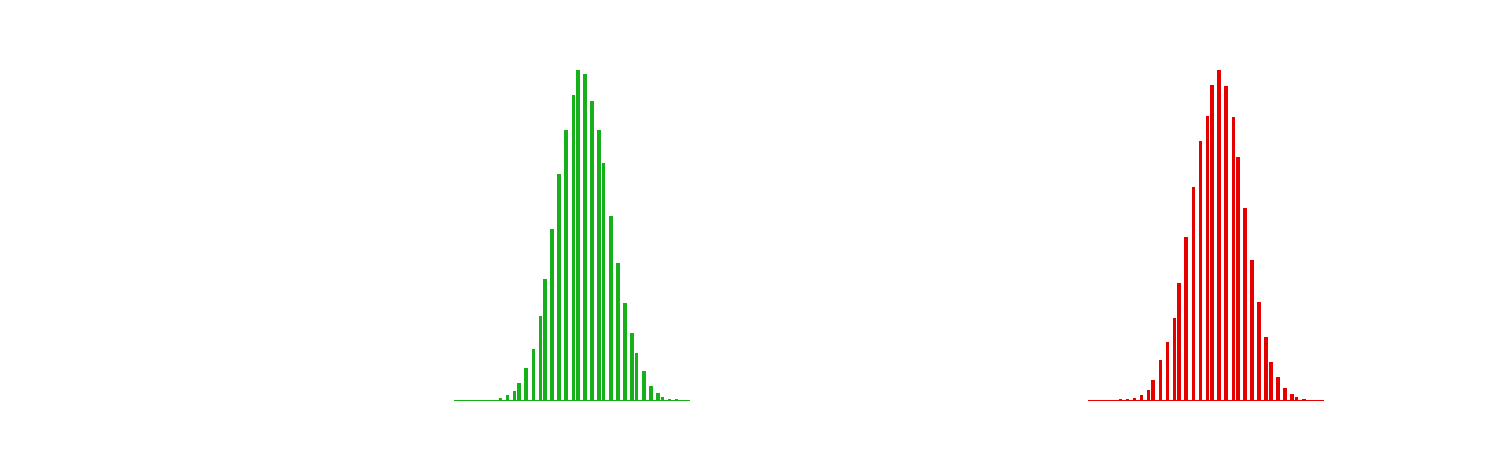
\includegraphics[width=\textwidth]{Results/3.5_boundariesBistability/maxReach0_0_HistogramPlot.pdf}
                    % \label{}
                \end{minipage}
            \end{minipage}
            \begin{minipage}{0.77\textwidth}
                \begin{minipage}{0.1\textwidth}
                    \caption*{\small \textbf{(b)}}
                \end{minipage}
                \begin{minipage}{0.66\textwidth}
                    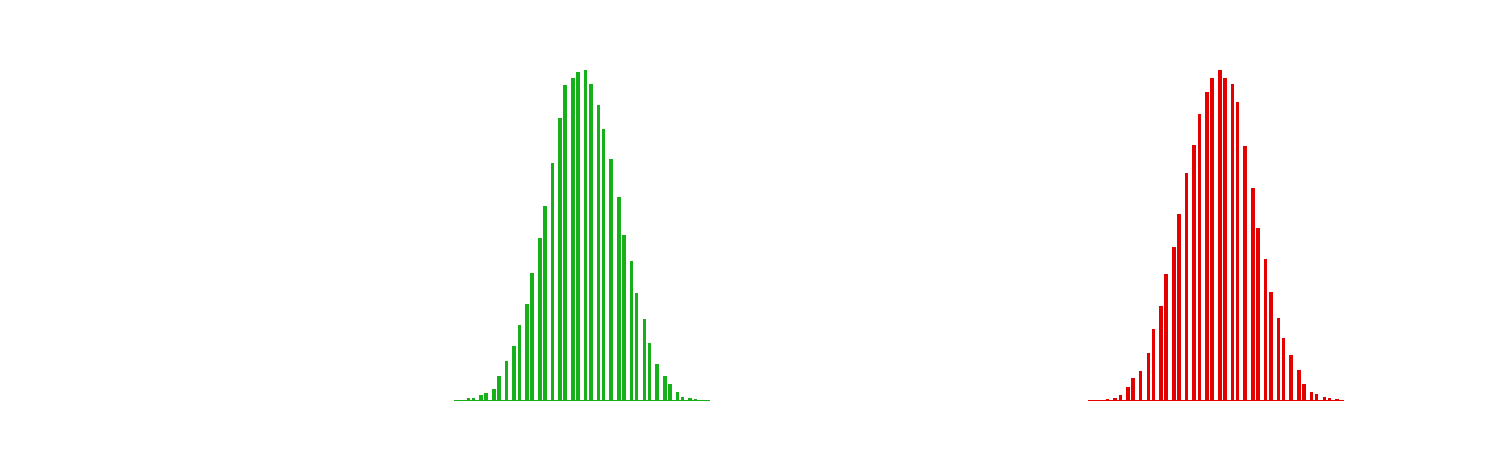
\includegraphics[width=\textwidth]{Results/3.5_boundariesBistability/maxReach1_4_HistogramPlot.pdf}
                \end{minipage}
            \end{minipage}
            \begin{minipage}{0.77\textwidth}
                \begin{minipage}{0.1\textwidth}
                    \caption*{\small \textbf{(c)}}
                    % \label{}
                \end{minipage}
                \begin{minipage}{0.66\textwidth}
                    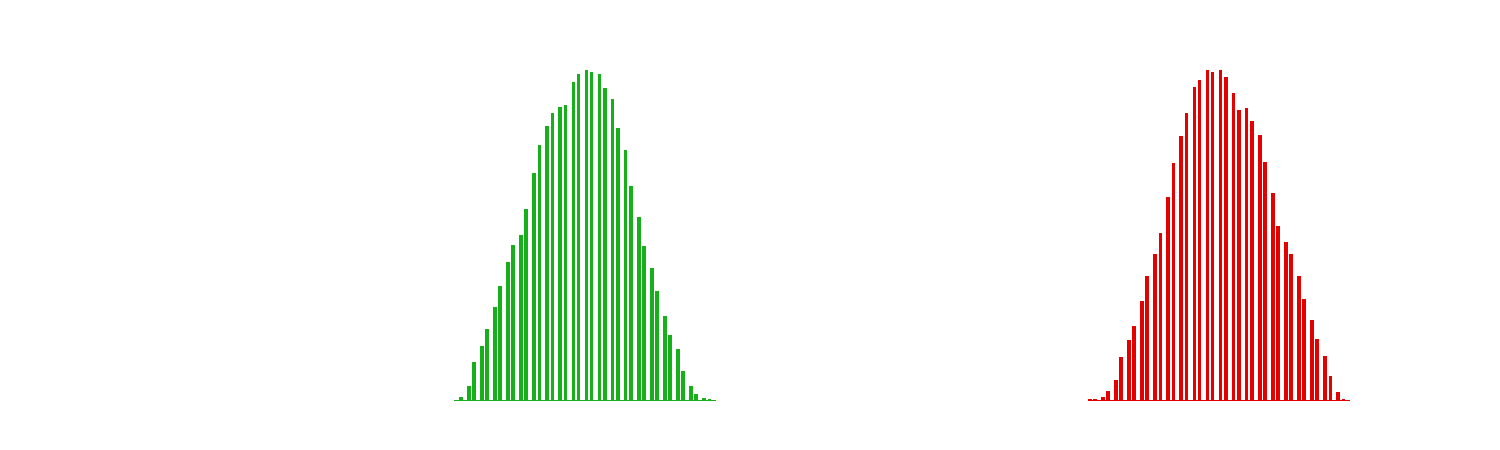
\includegraphics[width=\textwidth]{Results/3.5_boundariesBistability/maxReach2_2_HistogramPlot.pdf}
                    % \label{}
                \end{minipage}
            \end{minipage}
            \begin{minipage}{0.77\textwidth}
                \begin{minipage}{0.1\textwidth}
                    \caption*{\small \textbf{(d)}}
                \end{minipage}
                \begin{minipage}{0.66\textwidth}
                    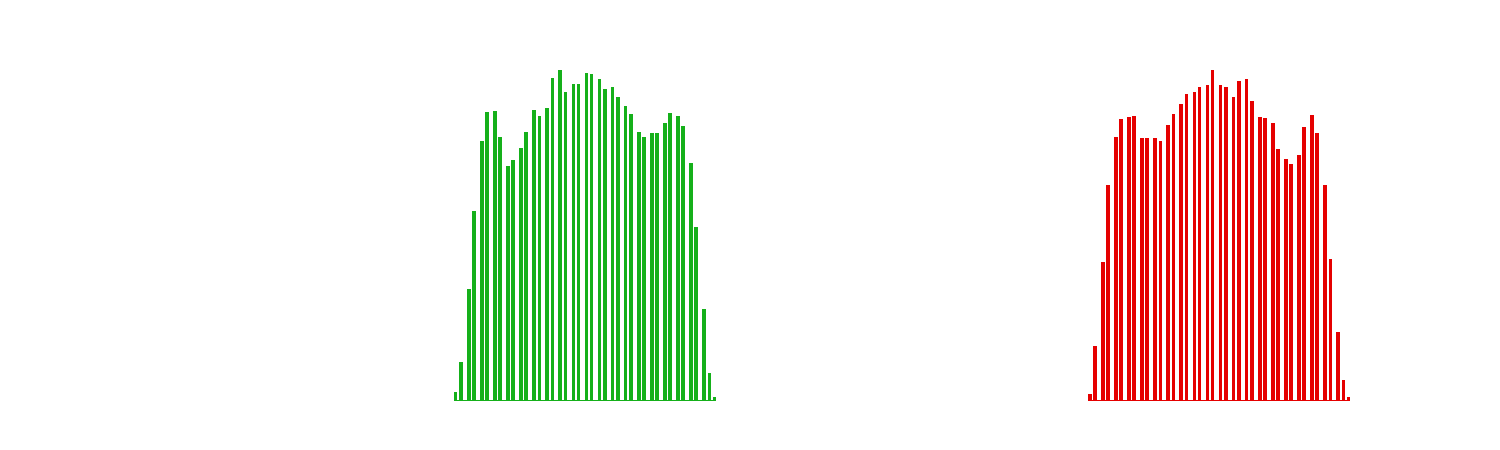
\includegraphics[width=\textwidth]{Results/3.5_boundariesBistability/maxReach3_3_HistogramPlot.pdf}
                \end{minipage}
            \end{minipage}
            \begin{minipage}{0.77\textwidth}
                \begin{minipage}{0.1\textwidth}
                    \caption*{\small \textbf{(e)}}
                    % \label{}
                \end{minipage}
                \begin{minipage}{0.66\textwidth}
                    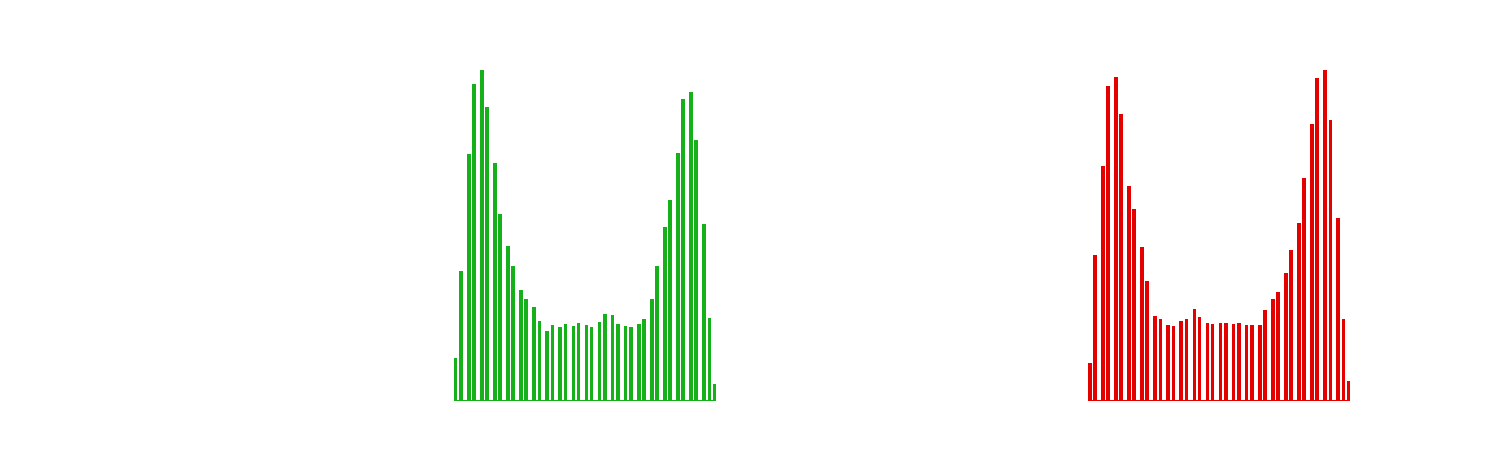
\includegraphics[width=\textwidth]{Results/3.5_boundariesBistability/maxReach4_3_HistogramPlot.pdf}
                    % \label{}
                \end{minipage}
            \end{minipage}
            \begin{minipage}{0.77\textwidth}
                \begin{minipage}{0.1\textwidth}
                    \caption*{\small \textbf{(f)}}
                \end{minipage}
                \begin{minipage}{0.66\textwidth}
                    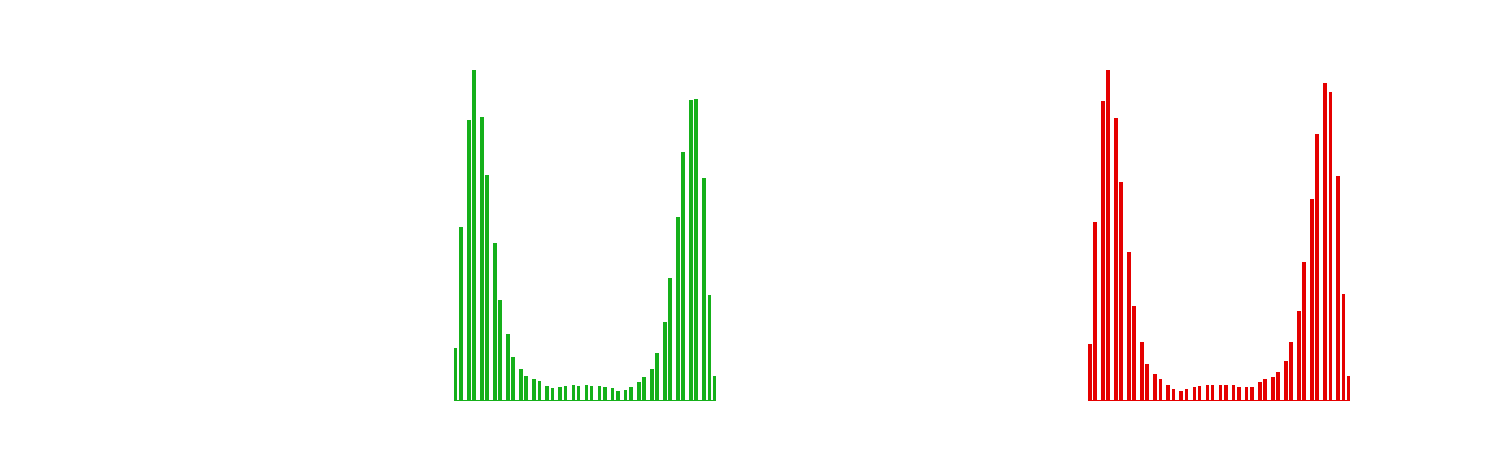
\includegraphics[width=\textwidth]{Results/3.5_boundariesBistability/maxReach5_4_HistogramPlot.pdf}
                \end{minipage}
            \end{minipage}
            \begin{minipage}{0.77\textwidth}
                \begin{minipage}{0.1\textwidth}
                    \caption*{\small \textbf{(g)}}
                \end{minipage}
                \begin{minipage}{0.66\textwidth}
                    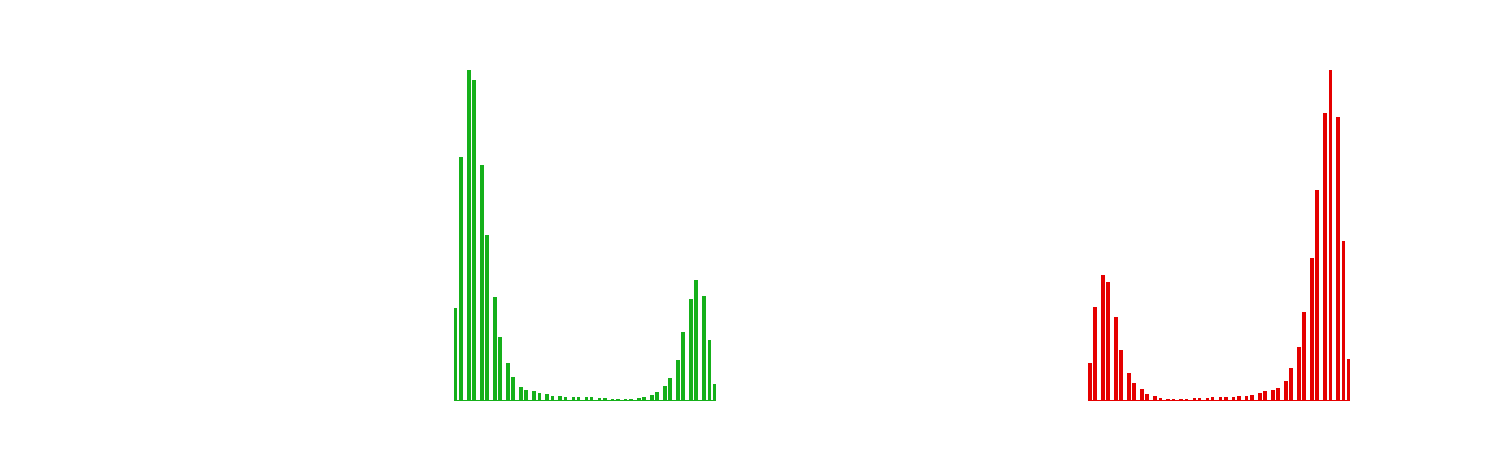
\includegraphics[width=\textwidth]{Results/3.5_boundariesBistability/maxReach6_4_HistogramPlot.pdf}
                \end{minipage}
            \end{minipage}
            \caption{}
            \label{img:enzymeReach}
        \end{figure}
        %
        \begin{itemize}
            {
                \color{red}
                \item describe loss of reach
                \item As can be seen in \textbf{(g)}, the symmetric case becomes more and more improbable because switching gets more rare and ?
            }
        \end{itemize}
        %
    %
    %
    \newpage
    \section{Bivalency}
        \label{sec:ResBivalency}
        %
        \begin{figure}[htpb!]
            \centering
            \includerunplot{Results/3.6_Bivalency/TotalComplete_example.png} % TODO change this
            \caption{}
            % \label{img:dissoc_runPlot2}
        \end{figure}
        %
        \begin{figure}[htpb!]
            \centering
            \includerunplot{Results/3.6_Bivalency/BivalentComplete_example.png} % TODO change this
            \caption{}
            % \label{img:dissoc_runPlot2}
        \end{figure}
        %
        \begin{figure}[htpb!]
            \centering
            \includerunplot{Results/3.6_Bivalency/BivalentBistability_example.png} % TODO change this
            \caption{}
            % \label{img:dissoc_runPlot2}
        \end{figure}
        %
        \begin{itemize}
            {
                \color{red}
                \item Here, we are at Kx+Ky
                \item Two systems that either favour bivalency or total active/silent states as an introduction to bivalency
                \item Frequent switching and bivalency
            }
        \end{itemize}
        %
    %
    %
%
%